% MILE procedure diagram, redrawn in TikZ from the draw.io source embedded in
% sommer2025_fig1_mile_flowchart.pdf (Sommer et al., ICLR 2025, Fig. 1; CC BY 4.0).
% Changes from the original: notation only -- network weights are w (theta is the
% SBI parameter in this report) and "parameter variances" -> "weight variances".
% Coordinates are the draw.io ones (pixels, y downward); 1 px = 0.727 pt as in the
% original PDF. Text in Helvetica (draw.io's default), math in Computer Modern
% (draw.io renders math with MathJax's TeX fonts).
% Build:  pdflatex mile_flowchart_ournotation.tex
\documentclass[border=1pt]{standalone}
\usepackage[T1]{fontenc}
\usepackage[scaled=0.92]{helvet}
\renewcommand{\familydefault}{\sfdefault}
\usepackage{amsmath,amssymb}
\usepackage{tikz}
\usetikzlibrary{arrows.meta}
\definecolor{bluefill}{HTML}{DAE8FC}\definecolor{bluestroke}{HTML}{6C8EBF}
\definecolor{orafill}{HTML}{FFE6CC}\definecolor{orastroke}{HTML}{D79B00}
\definecolor{greyfill}{HTML}{F5F5F5}\definecolor{greystroke}{HTML}{CCCCCC}
% font size and baseline skip in pt; no hyphenation inside the narrow text boxes
\newcommand{\pxfont}[2]{\fontsize{#1pt}{#2pt}\selectfont\hyphenpenalty=10000\exhyphenpenalty=10000}
\begin{document}
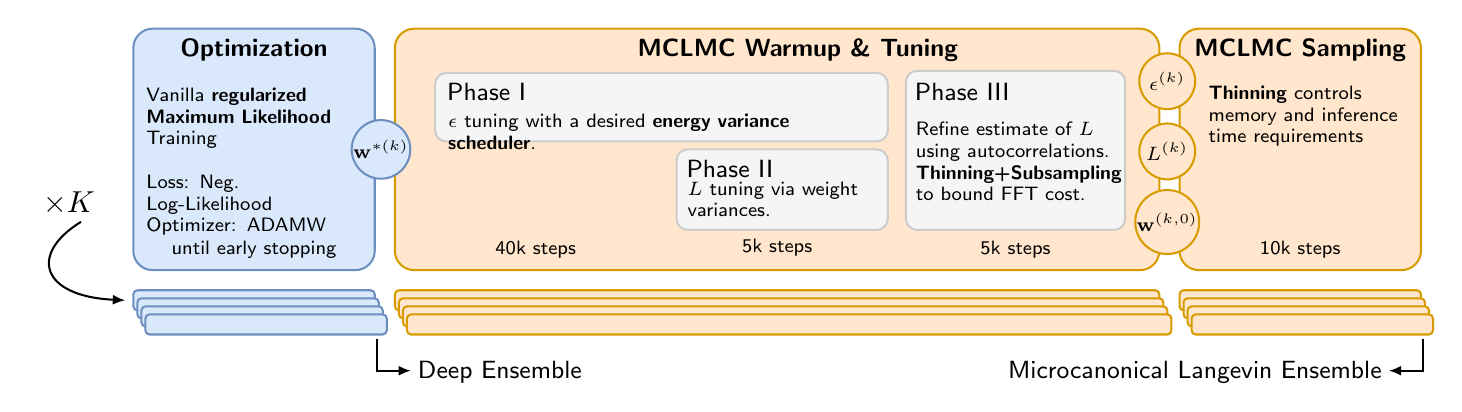
\begin{tikzpicture}[x=0.727pt,y=-0.727pt,line width=0.73pt,
  big/.style={rounded corners=7pt},
  mid/.style={rounded corners=4pt},
  bar/.style={rounded corners=1.5pt},
  body/.style={anchor=north west,align=left,inner sep=0pt,font=\pxfont{6.55}{7.85}},
  title/.style={anchor=center,align=center,inner sep=0pt,font=\pxfont{8.7}{10.4}\bfseries},
  phase/.style={anchor=west,inner sep=0pt,font=\pxfont{8.7}{10.4}},
  steps/.style={anchor=center,inner sep=0pt,font=\pxfont{7.3}{8.7}},
  label/.style={inner sep=0pt,font=\pxfont{8.7}{10.4}},
  circ/.style={circle,minimum size=20.2pt,inner sep=0pt,font=\pxfont{7.3}{8.7}},
  arr/.style={-{Latex[length=4.5pt,width=3.6pt]}}]

% stacked member bars (K copies), drawn back to front as in the original
\foreach \d in {0,2,4,6}{
  \draw[bar,fill=bluefill,draw=bluestroke] (150+\d,450+2*\d) rectangle ++(120,10);
  \draw[bar,fill=orafill,draw=orastroke]   (280+\d,450+2*\d) rectangle ++(380,10);
  \draw[bar,fill=orafill,draw=orastroke]   (670+\d,450+2*\d) rectangle ++(120,10);
}

% stage boxes
\draw[big,fill=bluefill,draw=bluestroke] (150,320) rectangle ++(120,120);
\draw[big,fill=orafill,draw=orastroke]   (280,320) rectangle ++(380,120);
\draw[big,fill=orafill,draw=orastroke]   (670,320) rectangle ++(120,120);

% phase boxes
\draw[mid,fill=greyfill,draw=greystroke] (300,342) rectangle ++(225,34);
\draw[mid,fill=greyfill,draw=greystroke] (420,380) rectangle ++(105,40);
\draw[mid,fill=greyfill,draw=greystroke] (534,341) rectangle ++(109,79);

% titles
\node[title] at (210,330.5) {Optimization};
\node[title] at (480.25,330.5) {MCLMC Warmup \& Tuning};
\node[title] at (730,330.5) {MCLMC Sampling};
\node[phase] at (305.5,351.5) {Phase I};
\node[phase] at (424.5,389.5) {Phase II};
\node[phase] at (538,351.5) {Phase III};

% body text
\node[body,text width=74.2pt] at (156,349) {Vanilla \textbf{regularized Maximum Likelihood} Training\\[7.85pt]
  Loss: Neg.\ Log-Likelihood\\ Optimizer: ADAMW};
\node[body,text width=152.7pt] at (306,362) {$\epsilon$ tuning with a desired \textbf{energy variance scheduler}.};
\node[body,text width=69.8pt]  at (425,395.5) {$L$ tuning via weight variances.};
\node[body,text width=70.5pt] at (538.5,366) {Refine estimate of $L$ using autocorrelations.\\
  \textbf{Thinning+Subsampling} to bound FFT cost.};
\node[body,text width=70.5pt]  at (684,348) {\textbf{Thinning} controls memory and inference time requirements};

% step counts
\node[steps] at (210,430)    {until early stopping};
\node[steps] at (350,430)    {40k steps};
\node[steps] at (470,429)    {5k steps};
\node[steps] at (588.5,430)  {5k steps};
\node[steps] at (730,430)    {10k steps};

% quantities carried between stages (circled)
\node[circ,fill=bluefill,draw=bluestroke] at (273.1,380)   {$\mathbf w^{\ast(k)}$};
\node[circ,fill=orafill,draw=orastroke]   at (663.9,346.1) {$\epsilon^{(k)}$};
\node[circ,fill=orafill,draw=orastroke]   at (663.9,381.0) {$L^{(k)}$};
\node[circ,fill=orafill,draw=orastroke]   at (663.9,416.1) {$\mathbf w^{(k,0)}$};

% x K loop and ensemble labels
\node[label,anchor=center,font=\pxfont{10.5}{12}] at (118,407) {$\times K$};
\draw[arr] (124,416) .. controls (98,432) and (104,453) .. (146,455);
\draw[arr] (271.3,474) -- (271.3,490) -- (288,490);
\node[label,anchor=west] at (291,491) {Deep Ensemble};
\draw[arr] (791,474) -- (791,490) -- (774,490);
\node[label,anchor=east] at (771,491) {Microcanonical Langevin Ensemble};
\end{tikzpicture}
\end{document}
